\chapter{Thuật toán DFS (tìm kiếm theo chiều sâu)}
\ifpdf
    \graphicspath{{Chapter3/Chapter3Figs/PNG/}{Chapter3/Chapter3Figs/PDF/}{Chapter3/Chapter3Figs/}}
\else
    \graphicspath{{Chapter3/Chapter3Figs/EPS/}{Chapter3/Chapter3Figs/}}
\fi


\section{Giới thiệu thuật toán}
DFS hay còn được gọi là tìm kiếm ưu tiên theo chiều sâu, tìm kiếm theo chiều sâu là một thuật toán duyệt trên một cây hoặc đồ thị. Thuật toán sẽ khởi đầu tại gốc hoặc một đỉnh bất kì (đỉnh này được xem như là gốc) và phát triển xa nhất có thể theo mỗi nhánh của gốc đó.\\
DFS là một dạng tìm kiếm thjoong tin không đầy đủ bởi vì quá trình tìm kiếm được phát triển tới đỉnh con đầu tiên của nút đang tìm kiếm cho tới khi gặp được đỉnh cần tìm hoặc tới một nút không có con. Khi đó giải thuật quay lui về đỉnh vừa mới tìm kiếm ở bước trước. Trong dạng không đệ quy, tất cả các đỉnh chờ được phát triển được bổ sung vào một ngăn xếp LIFO.
\\ Xét về độ phức tạp, theo không gian DFS sẽ thấp hơn BFS nhưng sẽ tương đương nhau khi xét về thời gian.
\section{Mô tả thuật toán}
Như hình dưới đây, thuật toán DFS sẽ bắt đầu tại đỉnh A và đi theo cạnh trái và tiếp tục tìm kiếm cho đến khi hết phần nhánh cây trái rồi mới chuyển sang nhanh con bên phải. Thứ tự sau khi chạy đủ thuật toán sẽ như sau: A, B, D, F,  C, G, E.\\

\begin{figure}[!htbp]
  \begin{center}
    \leavevmode
    \ifpdf
      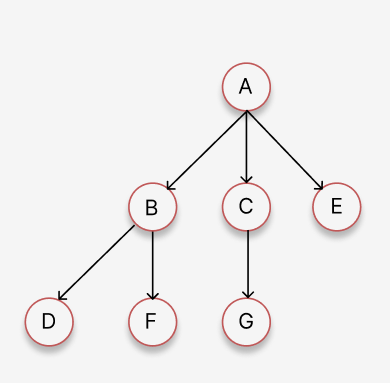
\includegraphics[height=3in]{DFS}
    \else
      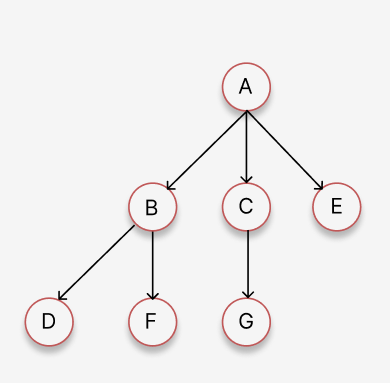
\includegraphics[bb = 92 86 545 742, height=6in]{DFS}
    \fi
    \caption{Cây đồ thị}
    \label{FigAir}
  \end{center}
\end{figure}

\section{Áp dụng thuật toán DFS vào bài toán sử dụng Prolog}
\subsection{Khởi tạo trạng thái đích}
\begin{figure}[!htbp]
  \begin{center}
    \leavevmode
    \ifpdf
      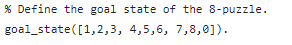
\includegraphics[height=0.5in]{DefineState}
    \else
      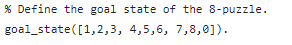
\includegraphics[bb = 92 86 545 742, height=0.5in]{DefineState}
    \fi
    \caption{Khởi tạo trạng thái đích}
    \label{FigAir}
   
  \end{center}
\end{figure}
\FloatBarrier
\subsection{Thuật toán DFS trong Prolog}
\begin{figure}[!htbp]
  \begin{center}
    \leavevmode
    \ifpdf
      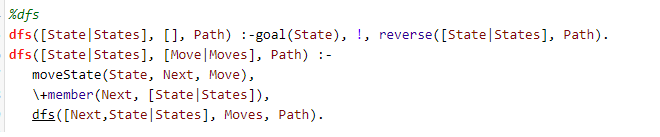
\includegraphics[height=0.5in]{DFS_function}
    \else
      \includegraphics[bb = 92 86 545 742, height=0.5in]DFS_function}
    \fi
    \caption{Thuật toán DFS trong Prolog}
    \label{FigAir}
   
  \end{center}
\end{figure}
\FloatBarrier
Thuật toán trên gồm ba tham số đầu vào là 'States', 'Moves' và 'Path'. Trong đó, 'States' là các danh sách cách trạng thái đã duyệt qua. 'Moves' là danh sách các thao tác di chuyển và 'Path' là đường đi xuất phát từ trạng thái khởi tạo đến trạng thái đích.
\subsection{Định nghĩa các hàm di chuyển}
Dưới đây là định nghĩa các thao tác di chuyển trong bà toán, trong đó '*' là ô trống. Mỗi hàm moveState sẽ nhận vào 1 trạng thái sẽ trả về một trạng thái mới sau khi di chuyển.
\begin{figure}
  \begin{center}
 \leavevmode
    \ifpdf
      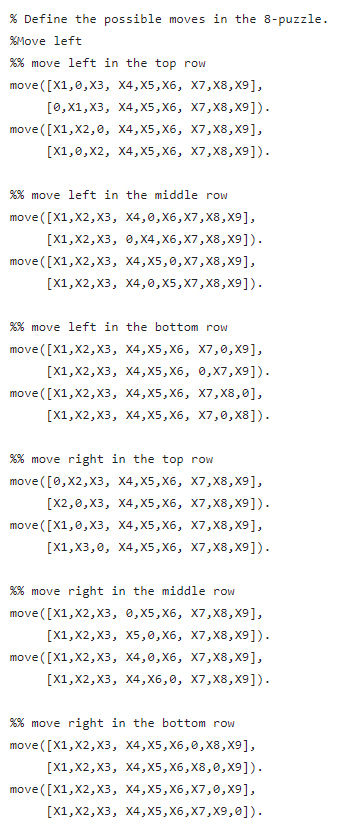
\includegraphics[height=5in]{MoveLeftRight}
    \else
      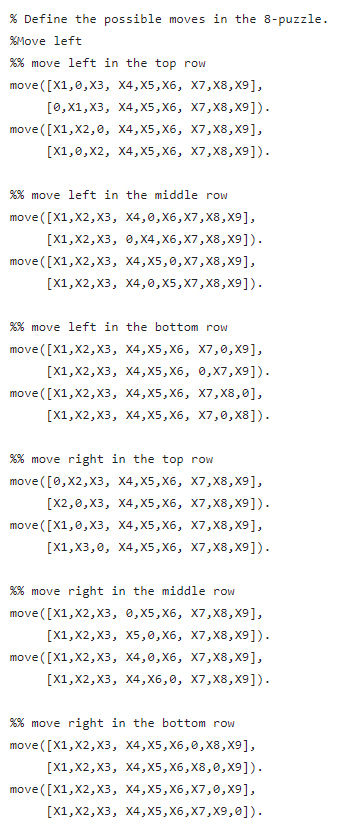
\includegraphics[bb = 92 86 545 742, height=5in]{MoveLeftRight}
    \fi
    \caption{Định nghĩa các hàm di chuyển}
    \label{FigAir}
 \end{center}
\end{figure}
\FloatBarrier

\FloatBarrier
\subsection{Cài đặt thuật toán và khởi chạy}
\begin{figure}[!htbp]
\begin{center}
    \leavevmode
    \ifpdf
      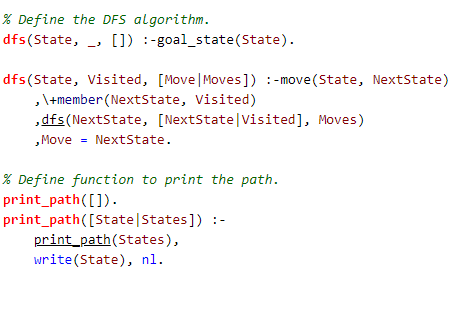
\includegraphics[height=3in]{Install}
    \else
      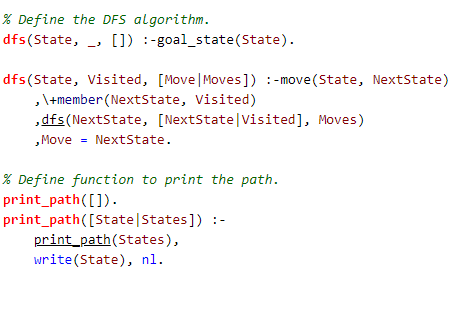
\includegraphics[bb = 92 86 545 742, height=3in]{Install}
    \fi
    \caption{Thuật toán DFS}
    \label{FigAir}
  \end{center}
\end{figure}
\FloatBarrier
Thuật toán bắt đầu bằng cách gọi hàm dfs với tham số đầu vào là danh sách chứa đỉnh xuất phát và danh sách rỗng để lưu các bước đi. Nếu đỉnh xuất phát là đỉnh đích, hàm sẽ trả về danh sách chứa đỉnh xuất phát. Nếu không, hàm sẽ lấy ra tất cả các đỉnh kề với đỉnh hiện tại, đánh dấu đỉnh hiện tại là đã thăm và gọi đệ quy lại hàm dfs để tiếp tục tìm kiếm đường đi. Nếu đường đi đã được tìm thấy, hàm sẽ trả về danh sách các đỉnh tạo thành đường đi từ đỉnh xuất phát đến đỉnh đích.\\
\subsection{Kết quả đạt được}
Kết quả đạt được sau khi chạy thuật toán.\\
\begin{figure}[!htbp]
\begin{center}
    \leavevmode
    \ifpdf
      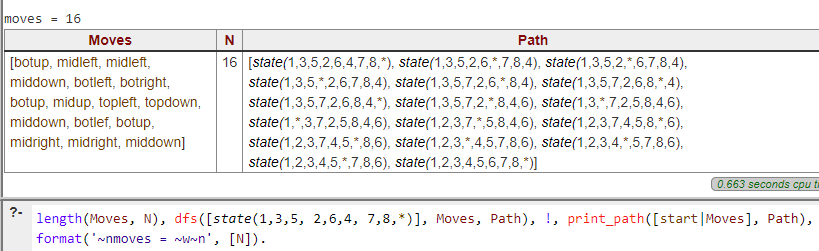
\includegraphics[height=2in]{Result}
    \else
      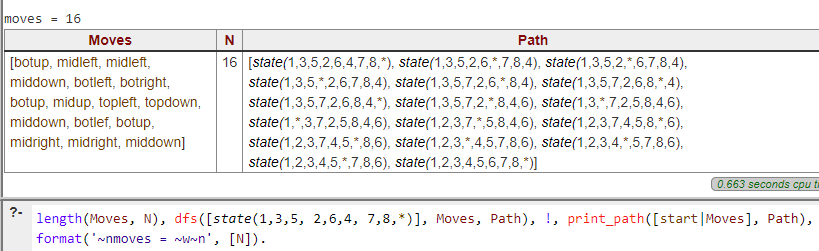
\includegraphics[bb = 92 86 545 742, height=2in]{Result}
    \fi
    \caption{Kết quả sau khi chạy}
    \label{FigAir}
  \end{center}
\end{figure}
\FloatBarrier


